\documentclass{amsart}
\usepackage[margin=1in]{geometry}

\usepackage{amssymb}
\usepackage{amscd}


\usepackage{graphics,amsmath,amssymb}
\usepackage{amsthm}
\usepackage{amsfonts}
\usepackage{latexsym}
\usepackage[pdftex]{graphicx}
\usepackage{float}
\usepackage{fancyhdr}

\pagestyle{fancy}
\lhead{Team \# 30698}
\rhead{\thepage}

\providecommand{\e}[1]{\ensuremath{\times 10^{#1}}}


\renewcommand{\refname}{}


\title{Traffic Flow and Safety Analysis Using a Discrete Particle Model \\ \vspace{1mm} {\small \textit{From a Hot Air Balloon Perspective}}}


\begin{document}
\DeclareGraphicsExtensions{.pdf,.png,.gif,.jpg}
\bibliographystyle{plain}
\maketitle

\tableofcontents


\newpage

\section{\bf{Introduction}}

	
	\subsection{Background}
		All countries implement a set of rules that help to regulate traffic and essential determine the common practices of the roads.  Many times though drivers choose to vary their compliance with all of these rules.  This disregard usually stems from drivers personal feelings on whether a rule is effective, if the rules conditions annoy the driver, and perceived time saved by breaking the rule.  One of these rules that has varying compliance is the rule that states a driver has to stay right unless to pass.  This states that a driver can only pass on the left of a driver and once they pass they should return to the right lane once they can.  Compliance is the key factor in the implications and effectiveness of this rule.  The question to be tested though is if people are going to follow this rule will it actually increase efficiency and safety of traffic flow. 
	
	\subsection{Approach}
		In order to test how efficient this rule is for traffic flow and safety, we needed to first establish a model for how our traffic is interacting and how the traffic is flowing as a whole. Essentially in order to test if the rule has an effect we cannot check already existing data but instead create our own data that is models a controlled variation in rule application. The currently most popular modeling of traffic involves treating the whole system as a pipe with fluid and then applying the discoveries and theorems of fluid dynamics.  This model is a macroscopic model though where essentially all control and measuring of the individual interactions is lost.  The other most common modeling technique for traffic flow is with individual particle interactions.  This treats each car, sometimes groups of cars, as a single particle and analyzing how these particles interact.  Our computer model turned out to be a particle model that treats each car as an individual.  Once we develop the system to analyze each individual interaction on a road system then we can begin to change how a driver will respond to this interaction.  As we vary these interaction choices, such as stay right except to pass or pass whenever and wherever you can, then we can see what the results of each interaction decision will have on the effect of the system as a whole.  

\section{\bfseries{Assumptions and Definitions}}
	\subsection{Definitions}
		\begin{itemize}
  			\item \textit{Highway}:an ideal model of a road with no entries or exit points
			\item \textit{Vehicle}:an ideal car that has all share same constant length 
			\item \textit{Driving Lane}: a highway lane a vehicle is free to travel in
  			\item \textit{Passing Lane}: a highway lane a vehicle can only travel in while passing
			\item \textit{Travel Time}: the time needed for a vehicle to travel length of road
			\item \textit{Traffic Flux}: the rate of cars passing a single location along the highway
			\item \textit{Rule}: distinct formulations of the passing laws 
			\item \textit{Side-Swipe Accident}: collision based solely on lane-changing
			\item \textit{Read-End Accident}: collision based solely on inefficiency to slow down
			\item \textit{Simulation Program}: the implementation of our model in  Object Oriented Programming Language
			
		\end{itemize}
	
	\subsection{Assumptions}
		General assumptions to the problem turned out to be one of the biggest road blocks that influenced our progress.  At each step in both the method choosing and the model developing we had to evaluate previous assumptions we had made and what further assumptions we would need to make in order to promote realistic situations while still having a solvable system.  There were some major overlaying assumptions that we made:
		\begin{itemize}
			\item  	Discrete Speed and Discrete Position
			\item  Hot Air Balloon Perspective
			\item 	All vehicles have the same length 
			\item 	Internal vehicular performance does not vary
			\item  Lane width, shoulder width, and curvature of road do not effect highway dynamics
			\item 	Conservation of Cars: Total Number of Cars on Road Constant
			
			\item  	All roads are uninterrupted highways
				\begin{itemize}
					\item 	No vehicles enter midway through road
					\item 	No stops in highway allowed (traffic lights/intersections) 
				\end{itemize}
			\item   Crashes have no effect on dynamics of highway
			\item 	Severity of Side Swipe accidents equal to severity of Rear-Ending accidents			
		\end{itemize}
		 

		To allow the model to be programmed we had to make the simplification that speed and positions of vehicles were both discrete quantities.  There are two reasons this is reasonable: snapshots of highway and ability to scale.  The discrete speeds and positions can be interpreted as snapshots of the highway at constant intervals.  This says that within our program each iteration is simply a snapshot of how the highway is performing at each period of time.  If we then scale the position spacing size down each iteration will represent smaller and smaller time periods.  This shrinking of time intervals is similar to the idea of a video being simply a sequence of photos changing at a fast speed.  As for speed, once we have discrete positions, speed can only be assigned in quantities of those discrete positions.  If position spacing was scaled down then velocity could be rescaled in terms of the new position interval in order to get more continuous velocity options. Furthermore, there is a lot of research on how very small deviations in speed can grow traffic jams quickly in places that wouldn't be expected \cite{kurttraffic}.  These phantom traffic jams will not appear in our model due to discrete speed.
	
		Hot Air Balloon Perspective is a perspective assumption based on a view of the whole section of the highway at a single time instead of an internal perspective where we are measuring from inside the system.  This plays into both the programming of the model as well as the macroscopic measuring of the system. 
		
		A constant vehicle length can be defined due to only slight variations in actual car length. Also, since there are discrete position intervals, a car can only be integer lengths of these discrete position intervals. As for modeling longer vehicles, the model can allow two constant length vehicles to be connected in line at a specific speed.

		Internal vehicular performance is in reference to that all cars break, accelerate, and function at equal levels.  This assumption is a more subtle point that would increase variable amount without increasing the benefit of testing the passing rules.  Also, by the assumption that cars travel at discrete constant velocities internal vehicular performance should not vary on a vehicle to vehicle basis. 

		Lane width, shoulder width, and curvature of the road are assumed to have no effect on the testing of the passing rules.  In general, lane widths on a highway have such small variations that any difference is assumed to have nominal effect on the ability to switch lanes.  Also, smaller lanes allow faster lane changes but decrease traveling safety so the assumption is these small variations do not affect safety. Same principles go apply to highway shoulders and median variations. No oncoming traffic is assumed so the median consideration is unnecessary at this time.  The median is taken to be so wide that the oncoming traffic has no effect on our vehicles decision making.  Shoulder width is seen to have an effect on a driver's safety perception in real analysis, but is assumed to have insignificant effect on the efficiency of a passing rule application \cite{elvik2009handbook}.
		 
		 Conservation of cars is a combination of factors: no vehicles enter mid-way through the highway and the density of the entire road as a whole is constant.  This correlates to there being no exit or entry ramps in this stretch of the highway and that as a car exits the highway a car enters the highway.  This assumption is essentially a simplification for programming the model because we need a way to add new cars to the highway but generating new cars after each iteration would not provide enough benefit for the use of our programming time frame. As the length of the highway is increased though the inaccuracies decrease because it takes longer for a car to pass the same vehicle twice.  To further justify this assumption reference can be made to large percentage of traffic models that do in fact make this assumption \cite{seiboldconstructing}.  
		 
		 In our definition of a highway the assumption was already made that there are no exits or entry ramps midway through the highway.  Further we want to exclude any slowing or stopping due to traffic lights, intersections, or further impairments since these should not have an effect on the specific testing of the passing rules.  Our model allows for these adjustments to be made with minimal code writing but once again the time to write it would not be beneficial enough to test these specific passing rules.  

		In our model we calculate the amount of accidents that are likely to result on a highway but simultaneously assuming that a crash will not stop or slow down traffic.  One main reason for this assumption is to make the programming simpler, since an accident is simply a number count in the program.  More importantly though, the assumption is justified because we want to test crashes caused simply by these passing rules.  When crashes are allowed to slow down traffic, the model begins to add accidents do to the slowing and increasing density of traffic and not directly the passing rules themselves.  

	Although there are different probabilities associated with side-swipe accidents vs. read-end accidents no severity of crash time is assigned.  That implies that the safety of the highway is not associated with how bad accidents on the highway actually are.  This could be later factored in but there are too many variables to associate a severity of an accident to program a severity calculator in this time.  This assumption is also reasonable because even non-severe accidents should  be prevented. 
		


\section{\bfseries{Development of Method}}
	\subsection{Method Rational}
	Our approach to testing passing rules was to develop an effective model for traffic interactions that could create it's own data depending on the set of rules for the road that we wanted implicated.  This would then allow more control over parameter variation instead of simply relying on already collected data by others for a specific highways with a specific rule.  Furthermore, if we were able to build a model that had very specific parameter variation capabilities then the analysis of the road rules would be easier to analyze and interpret since we could run rules against control situations.  
	
	
	
	Initially there were three general model ideas that we considered in order to create these rule data variations. The first was a single particle model that would effectively model each individual interaction of a car trying to pass another car.  The other extreme was the macroscopic idea, modeling the highway as a whole, to use differential equations to model the rate of flow for traffic.  Inside the idea of differential equations, fluid dynamics and it's associated differential equations were discovered to be of significant current use in modeling traffic flow.  The third model we considered developing was some form of a combination of the particle model and fluid dynamics model \cite{burghout2005}.
		
		\subsubsection{\it Fluid Dynamics}
		In the realm of macroscopic traffic modeling, fluid dynamics is the most popular and common technique.  The idea behind this technique is that cars in heavy traffic interact similar to particles, either gas or liquid, in a confined tube.  
The difference between gas and liquid being the property of compressible, or the ability to change density of the fluid.  A gas model is said to be compressible, allowing changes in  fluid density.  While a liquid model is said to be incompressible, allowing no change in fluid density \cite{stone2007introduction}.  The majority of fluid dynamical models that we considered used incompressible calculations on both a macroscopic and microscopic model.  Our first approaches involved attempting to vary viscosity within the fluid and vary the shape of the tube the fluid traveled through.  By varying viscosity then the high viscosity pockets of fluid would represent slow pods of traffic while low viscosity fluid would represent fast moving pods of traffic.  The other technique called slow traffic pods an actual unmovable obstruction as part of the pipe wall or shape.  
		
		
	
	
	
		
		\subsubsection{\it Discrete Particle Model}
		
	The other extreme of modeling that we tried to pursue involved a discrete particle model that monitored individual interactions.  In this model we were hoping to create a program in detail that modeled specific passing characteristics of interactions.  By evaluating the actual different parameters that make up every passing interaction then these would shed light on the efficiency of the stay right except passing rule.  This model would be able to measure the safety of passing on the right vs. passing on the left, amount of time required for each passing interaction, the effect passing had on the immediate properties of each vehicle, etc.  
	Within this model though you start to lose sight of the overall highway as a whole.  By simply considering a few interactions at a time it is almost impossible to see traffic jams develop, highway flow changes, or density of the highway.  If we could not test these factors then it would be hard to say whether the different passing rules had any large effect on the efficiency of the highway system as a whole.  
		
		\subsubsection{Mixed Model}
		
	Eventually the obvious conclusion was to attempt to find an effective median between macroscopic fluid dynamics and the individual discrete particle model.  Along with this though we decided to start with the discrete particle model and slowly generalize it into a more macroscopic situation.  By utilizing the particle model still we had an effective way to vary the actual interaction between every single car.  This gave us complete control over what actually happens when a car tries to pass another car.  
	
	The very first model that we fully developed was a short programming code that gave us data we could then illustrate on graph paper.  This original program only had a road length of 100 tiles, with discrete tile position and speed based off of tiles per iteration of the program.  As we drew out the positions we began to discover not only the bugs in our program program but also in the short length of road and vehicular speed classes of 1,2,3 tiles/iteration.  We were able to further understand which aspects of each passing interaction we considered the most important and these began the factors of test in our final method.  

	\subsection{Discrepancies of Fluid Dynamics}
	The major problem right away with fluid dynamical modeling was creating a solution to implement a passing rule into the fluid's attributes. Since we were unsuccessful in finding an already existing model that allowed for this variation in passing rule, the technique we pursued was implementing a system containing a fluid with non-unified viscosity. 
	
	One problem that appeared with using fluid dynamical techniques was the models accuracy to model traffic decreases as density decreases \cite{stone2007introduction}.  This is in effect because as density decreases there begins to appear these large gaps in traffic that would not be present in either a liquid or a gas, even if we allowed the fluid to be a compressible fluid.  One variation in parameters that we consider important for testing was the passing rules efficiency in both low and high density. Some models attempted to adjust for density by varying viscosity of the fluid as we had hoped.  In these cases though the differential equation analysis became more and more complicated as the viscosity varied.  Since we felt our model required large variations in viscosity in small intervals we were led to the conclusion that all these models assumptions generalized the fluid into too macroscopic of a model to test any passing rule interaction of vehicles effectively.    

	We further investigated other theories in the fluid model however found that simply none allowed the use of a particle specific rule that we felt comfortable enough quantifying as a passing rule, thus preventing us from using them to answer the basic problem statement \cite{piccolireview}.
	

\section{\bfseries{Road Rules}}
	The rule that staying right except to pass becomes a more subtle point as the highway becomes three or more lanes wide.  Essentially there are two different rules that this stay right rule breaks down into when three or more lanes are present.  There is the rule that all drivers must remain as far right as possible and the rule that there is a single left most passing lane and drivers can travel within the remain other lanes freely.  In order to test all variations in passing tendencies four separate passing rules were developed:
		\begin{itemize}
			\item No Passing Allowed
			\item Free Passing
			\item Single Passing Lane
			\item Single Driving Lane
		\end{itemize}
	These are the four different rules of passing that we decided to test within our model.

	\subsection{No Passing Allowed}
	The No Passing Allowed Rule states that all lanes on the highway are driving lanes and that there is no passing involved in the system at all.  Under this rule whatever lane a vehicle starts within the vehicle will remain in that lane for the entirety of its travel.  The obvious result of this system is that quickly there will be large chains of cars all going at the same speed.  When the two or more lanes are present on a stretch of highway this model has no practical application, which supports why we are developing it as a control rule.  There are applications to this rule though when the highway only has one lane traffic, as in a construction zone or on a highway where there is only one lane traffic in each direction and the oncoming traffic is too heavy to ever pass.  In these cases, this No Passing Allowed Rule can provide effect insight into the clustering of these speed pockets.  Our research question is not concerned with this case of speed pockets though so we will simply think of this No Passing Allowed Rule as a base case that represents an extreme in the spectrum of rules.  
	\subsection{Free Passing}
	The Free Passing Rule states that the vehicle will continue in its current lane until it approaches another vehicle in its lane.  At the point that another vehicle is in front of the target vehicle the target vehicle will attempt to change lanes.  The vehicle will first try to pass the front vehicle on the left, but if there is no lane open to the left then the vehicle will attempt to also pass to the right.  If passing is also not possible to the right then the car will slow down to mirror the speed of the vehicle it is following. 

	Therefore there are two important differences in this rule then in the other rules, direction of passing and the action after lane changing.  Under this rule vehicles can pass going either to the left or to the right.  Also, once a vehicle does change lanes it will remain in that lane until it is forced to pass again.  

	This rule is providing us with a model that shows the absence of any passing laws.  In practical application most cars do not operate by this Free Passing Rule, but there are certain individuals who interact in this manner when they feel they need to.  The real importance of this rule is that it provides a control case on the other extreme of the rule spectrum opposite that to the No Passing Rule.  The Free Passing Rule says that there is an absence of any rules regarding passing and thus gives a basis to show that passing rules need to be implemented to improve efficiency and safety. 
	
	\subsection{Single Passing Lane}
	The Single Passing Rule states that there is only a single passing lane on the multilane highway and the remaining lanes are designated as driving lanes.  A Single Passing Rule and a Single Driving Rule are equivalent on a one or two lane highway.  This rule was created in order to account for the travel of slower vehicles in more than just the farthest right lane for highways of more than two lanes.  Therefore any lane that is not the farthest right or the farthest left lanes allows both driving and passing within it. 
	
	This rule can be assumed to closed mirror how heavy traffic flow works on a busy multilane highway.  Drivers tend to spread out among multiple lanes spending more time in a lane the farther right that lane is on the highway and leaving the left lane frequently empty or for carpooling.  We have not including any regard for a carpool lane since in our program only fast drivers will be traveling in the left lane at any time.   
	
	\subsection{Single Driving Lane}
	The Single Driving Rule states that the farthest right lane is a driving lane and all other lanes on the highway are only passing lanes.  A Single Driving Rule and a Single Passing Rule are equivalent on a one or two lane highway.  

	This rule tests the stay right except to pass law most efficiently.  By forcing drivers to only travel in the right lane except while passing the system takes into effect that a vehicle has to return to the same lane they were previously traveling in before overtaking another vehicle. Therefore this rule must be tested against the efficiency and safety of all the other rules in order to actually test the stay right except to pass law.    

\section{\bfseries{Modeling}}

\textit{\textbf{Model Specific Definitions}}

\begin{itemize}
	\item \textit{Initial Speed}: speed of individual vehicle at start of simulation
	\item \textit{Current Speed}: speed of individual vehicle at individual time	
	\item \textit{Iteration Average Speed}: the average current speed of all vehicles on the highway
	\item \textit{Highway Density}: amount of cars over whole highway; constant in current model
	\item \textit{Traffic Flux}: the average speed multiplied by the highway's density
	\item \textit{Road Type}: initial conditions of a highway based on density (high or low) and lane count (2-5)
	\item \textit{Simulation}: total iterations for all possible road type	
	\item \textit{Average Simulation Speed}: the average speed for a certain road type simulation
	\item \textit{Simulation Iteration}: distinct interval of time represented by each iteration
	\item \textit{Simulation Parameters}: the programs initial requested variables: number of simulation, passing rule, number of roads, length of road, iterations per simulation
	\item \textit{Summary Data}: output data for program: lane count, traffic density, average speed, total slow downs, total lane changes, total decisions
	\item \textit{Road Summary Data}: summary data for an individual road type after each iteration
	\item \textit{Simulation Summary Data}: summary data for each simulation as a whole
	\item \textit{Safety Rating}: scaled probability of an accident during a simulation
	\item \
\end{itemize}
	
\textit{\textbf{Model Specific Assumptions}}

	\begin{itemize}
	\item Normal Distribution of Initial Speed
	\item Speed Increases to Initial Speed When Possible
	\item Mirrored Traffic Assumption	
	\item All overlying assumptions stated previously.
	
\end{itemize}

\textit{Justifications}\\


	
	
	
	Initial speed of the vehicles on the highway was chosen by a normal distribution.  This assumption was actually made to maximize the realism of our method.  Speeds in the current scaling of the system are taken to range from 54 MPH to 90 MPH.  This sets the average speed of the highway at 70 MPH which is a common speed limit for United States highways.  By normally distributing initial speeds the break downs are:
	
	

	Inside the simulation vehicles are often slowing down since no crashes are allowed in the system.  Therefore we assume that every vehicle wants to accelerate back to it's initial speed as soon as it possibly can.  This is an important assumption in the realism of the method because on real highways individual drivers tend to drive at a steady average speed when their path is not impeded.  
	
	We are making the assumption that traffic that drives on the left side of the road is simply a mirror image of traffic that drives on the right side of the road, such as in the United States. Thus, staying right except to pass on the left is the same as staying left except to pass on the right. Additionally, switching lanes to the left is assumed to be the same as switching lanes on the right.
	
	

	
	\subsection{Implementation of Model}
	

		\subsubsection{Why Java and XML?}
			We chose to implement our traffic model using Java for two main reasons. We wanted to use a language that allowed us to encapsulate our model in a class structure. Thus, the high-level language and object-orientated structure of Java was our foremost reason for implementing our model in Java.  Additionally, we chose Java over other object-orientated, high-level languages because our familiarity with programming in Java out-weighed our desire to learn the ins-and-outs of an unfamiliar high-level language. \\
			As for the persistence of our simulation summary data, we chose to use the data persistence functionality of Extensible Markup Language (XML) because of the ability within Java to easily convert data encapsulated in our class structure to XML data encapsulated in Java packages that handle Java-to-XML interactions. Furthermore, XML is a standard data persistence language that easily imports into many different types of data analysis software, such as Microsoft Excel.  
		\subsubsection{Encapsulation of Model with Object Orientation}
		As mentioned above, we wanted to make use of object orientation to encapsulate our model into a class structure. Due to time constraints we minimized the class structure of our simulation program to include only the functionality and data encapsulation necessary to fully implement our model. Below is a breakdown of the functionality and data encapsulation for each class in our program.
		\begin{enumerate}
			\item{\textbf{\texttt{Car}}
				This class encapsulates the initial speed of a car, determined by our normal distribution of car speeds, the current speed of a car, changed by our logic tree (see Figure ~\ref{MCM-LogicalFlowChart}.), and the passing state of a car, either true of false. 
			}
			\item{\textbf{\texttt{DataPersistence}}
				This class encapsulates the functionality for persisting the simulation summary data into an XML file. This class handles the conversion of the encapsulation of the simulation summary data to data in an XML file using \texttt{java.io.*}, \texttt{java.xml.*}, \texttt{org.w3c.dom.*} packages.
			}
			\item{\textbf{\texttt{Main}}
				This class is the entry point for the flow of execution of our simulation program. The interface for prompting a user for the simulation parameters and looping structure for running multiple simulations with the same parameters are encapsulated in this entry-point class.
			}
			\item{\textbf{\texttt{Map}}
				This class encapsulates a collection of roads that a simulation tests. Each road in the \texttt{Map} represents a different road type that the simulation tests with a specific rule.
			}
			\item{\textbf{\texttt{Position}}
				This class encapsulates a position on a road by the lane and slot (length-wise position) values.
			}
			\item{\textbf{\texttt{Road}}
				This class encapsulates the properties of a road in our simulation, based on our assumptions. These properties include the number of lanes, the length of the road, the traffic on the road (i.e., a collection of cars), and counts of the number of decisions, lane changes and slow downs that occurred during an iteration of our simulation program. Since our model assumes a hot air perspective, the array used to store the cars on a road has the dimensions of road, as seen from a hot air balloon, and the position of each car (in terms of lane and slot) are the indices of the car object in the array.
			}
			\item{\textbf{\texttt{Rules}}
				This enumerator class encapsulates a designation of the rule used to navigate our logic tree (see Figure ~\ref{MCM-LogicalFlowChart}.) during a simulation. The values stored in this enumerator class are \texttt{FREE PASSING, SINGLE PASSING, SINGLE DRIVING, NO PASSING}.
			}
			\item{\textbf{\texttt{Simulation}}
				This class encapsulates a collection of different road types that different numbers of lanes and different traffic densities to test how these parameters, in conjunction with a rule, affect the flow of traffic on a road type.
			}
			\item{\textbf{\texttt{SummaryData}}
				This class is an abstraction of vector that is used to store the summary data the we use in our statistical analysis. All of the variables defined as our summary data are encapsulated as private fields in this class.
			}
		\end{enumerate}
		
\newpage

		\subsubsection{Program Execution Flow}		
			Now that we have discussed the overall class structure of our simulation program, we can explain the flow of execution of our simulation program. At the entry point of our simulation program, the user is prompted for the simulation parameters. Then, for each simulation specified by the number of simulations to run, our simulation program creates a new instance of the \texttt{Simulation} class and runs that simulation instance by calling the public instance method \texttt{Run()}. Next, within this public instance method (of the \texttt{Simulation} class), the collection of roads are generated and populated cars. The position of a car is randomly generated using a uniform distribution, and the speed of a is randomized using our normal distribution model for possible car speeds. After the roads have been populated with random cars, our simulation program begins looping through the number of iterations defined in the simulation parameters. Within each iteration, our simulation program implements our logic tree (see Figure ~\ref{MCM-LogicalFlowChart}.) to calculate new positions for each car on each road. As soon as the execution of our logic tree finishes, our simulation program calculates the summary data for each road. Recall that each road in a simulation represents a different road type. After the simulation program finishes computing all the iterations specified by the simulation parameters, then the summary data for the whole simulation is calculated. At this point the simulation program is done computing iterations, so the simulation summary data is persisted in an XML file using an instance of the \texttt{DataPersistence} class. Finally, if there are multiple simulations defined by the simulation parameters, the simulation program iterates to the next simulation instance. (see Figure ~\ref{MCMProgramFlow}.)
		
		
			
		\subsubsection{Flaws and Improvements}
			Overall, the simulation program we developed implemented our model better than anticipated, especially within the time constraints. However, overall design flaws produced issues with the collection, persistence, and analysis of the simulation summary data. Initially, we attempted to collect and persist data for every car on every road during every simulation. This method of collecting and persisting \emph{all} data would have required terabytes of storage space, which we did not have access to, nor time to analyze. So, we changed the way in which we collected and persisted data so that only the summary data for each iteration was stored in output XML file. However, we encountered several problems, mostly from time limitations, trying to import and analyze the data in Microsoft Excel. Thus, due to time constraints, we decided to only output summary data for each simulation. Therefore, when we continue to investigate this problem, we plan to use a database, instead of XML files, to persist our traffic data. A database would allow our simulation program to persist more information with an organizational structure that makes the statistical analysis of the data easier. Additionally, using a database to persist more data with better organization, would allow us to develop an extension of our simulation program that plays back the movement of traffic our simulation program calculated. This extension would allow us to analyze the traffic flow visually, instead of purely analytically. This would present us with the opportunity to catch further design flaws in both our model and implementation of the model.	
			
\newpage
			
	\begin{figure}[H]
	\begin{center}
	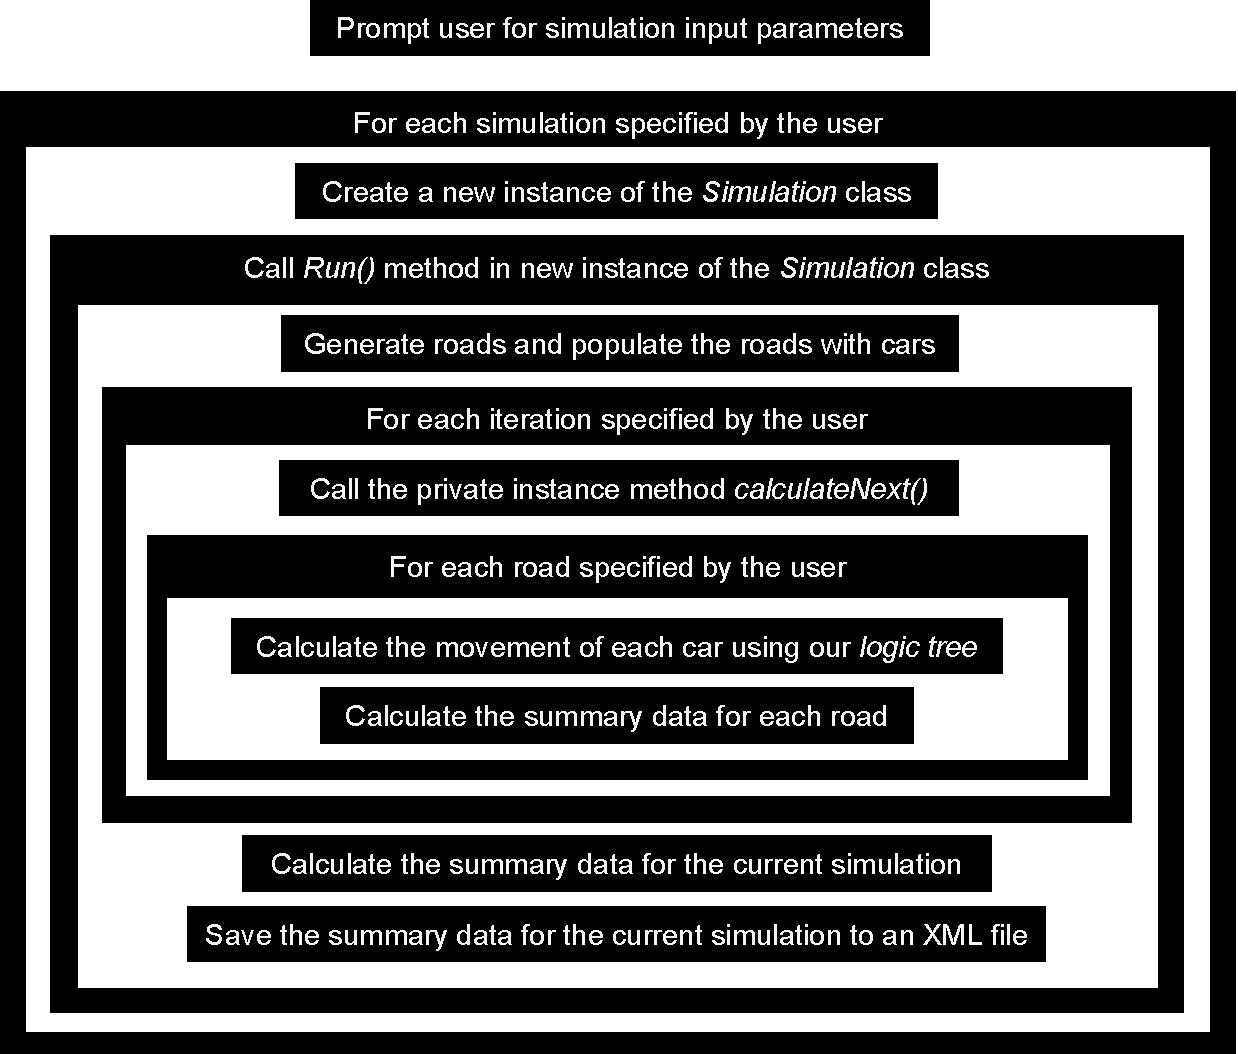
\includegraphics[scale=0.49]{MCMProgramFlow}
	\caption{The Flow of Execution of the Simulation Program}
	\renewcommand{\figurename}{}
	\label{MCMProgramFlow}
	\end{center}
	\end{figure}		
	
	
	\begin{figure}[H]
	\begin{center}
	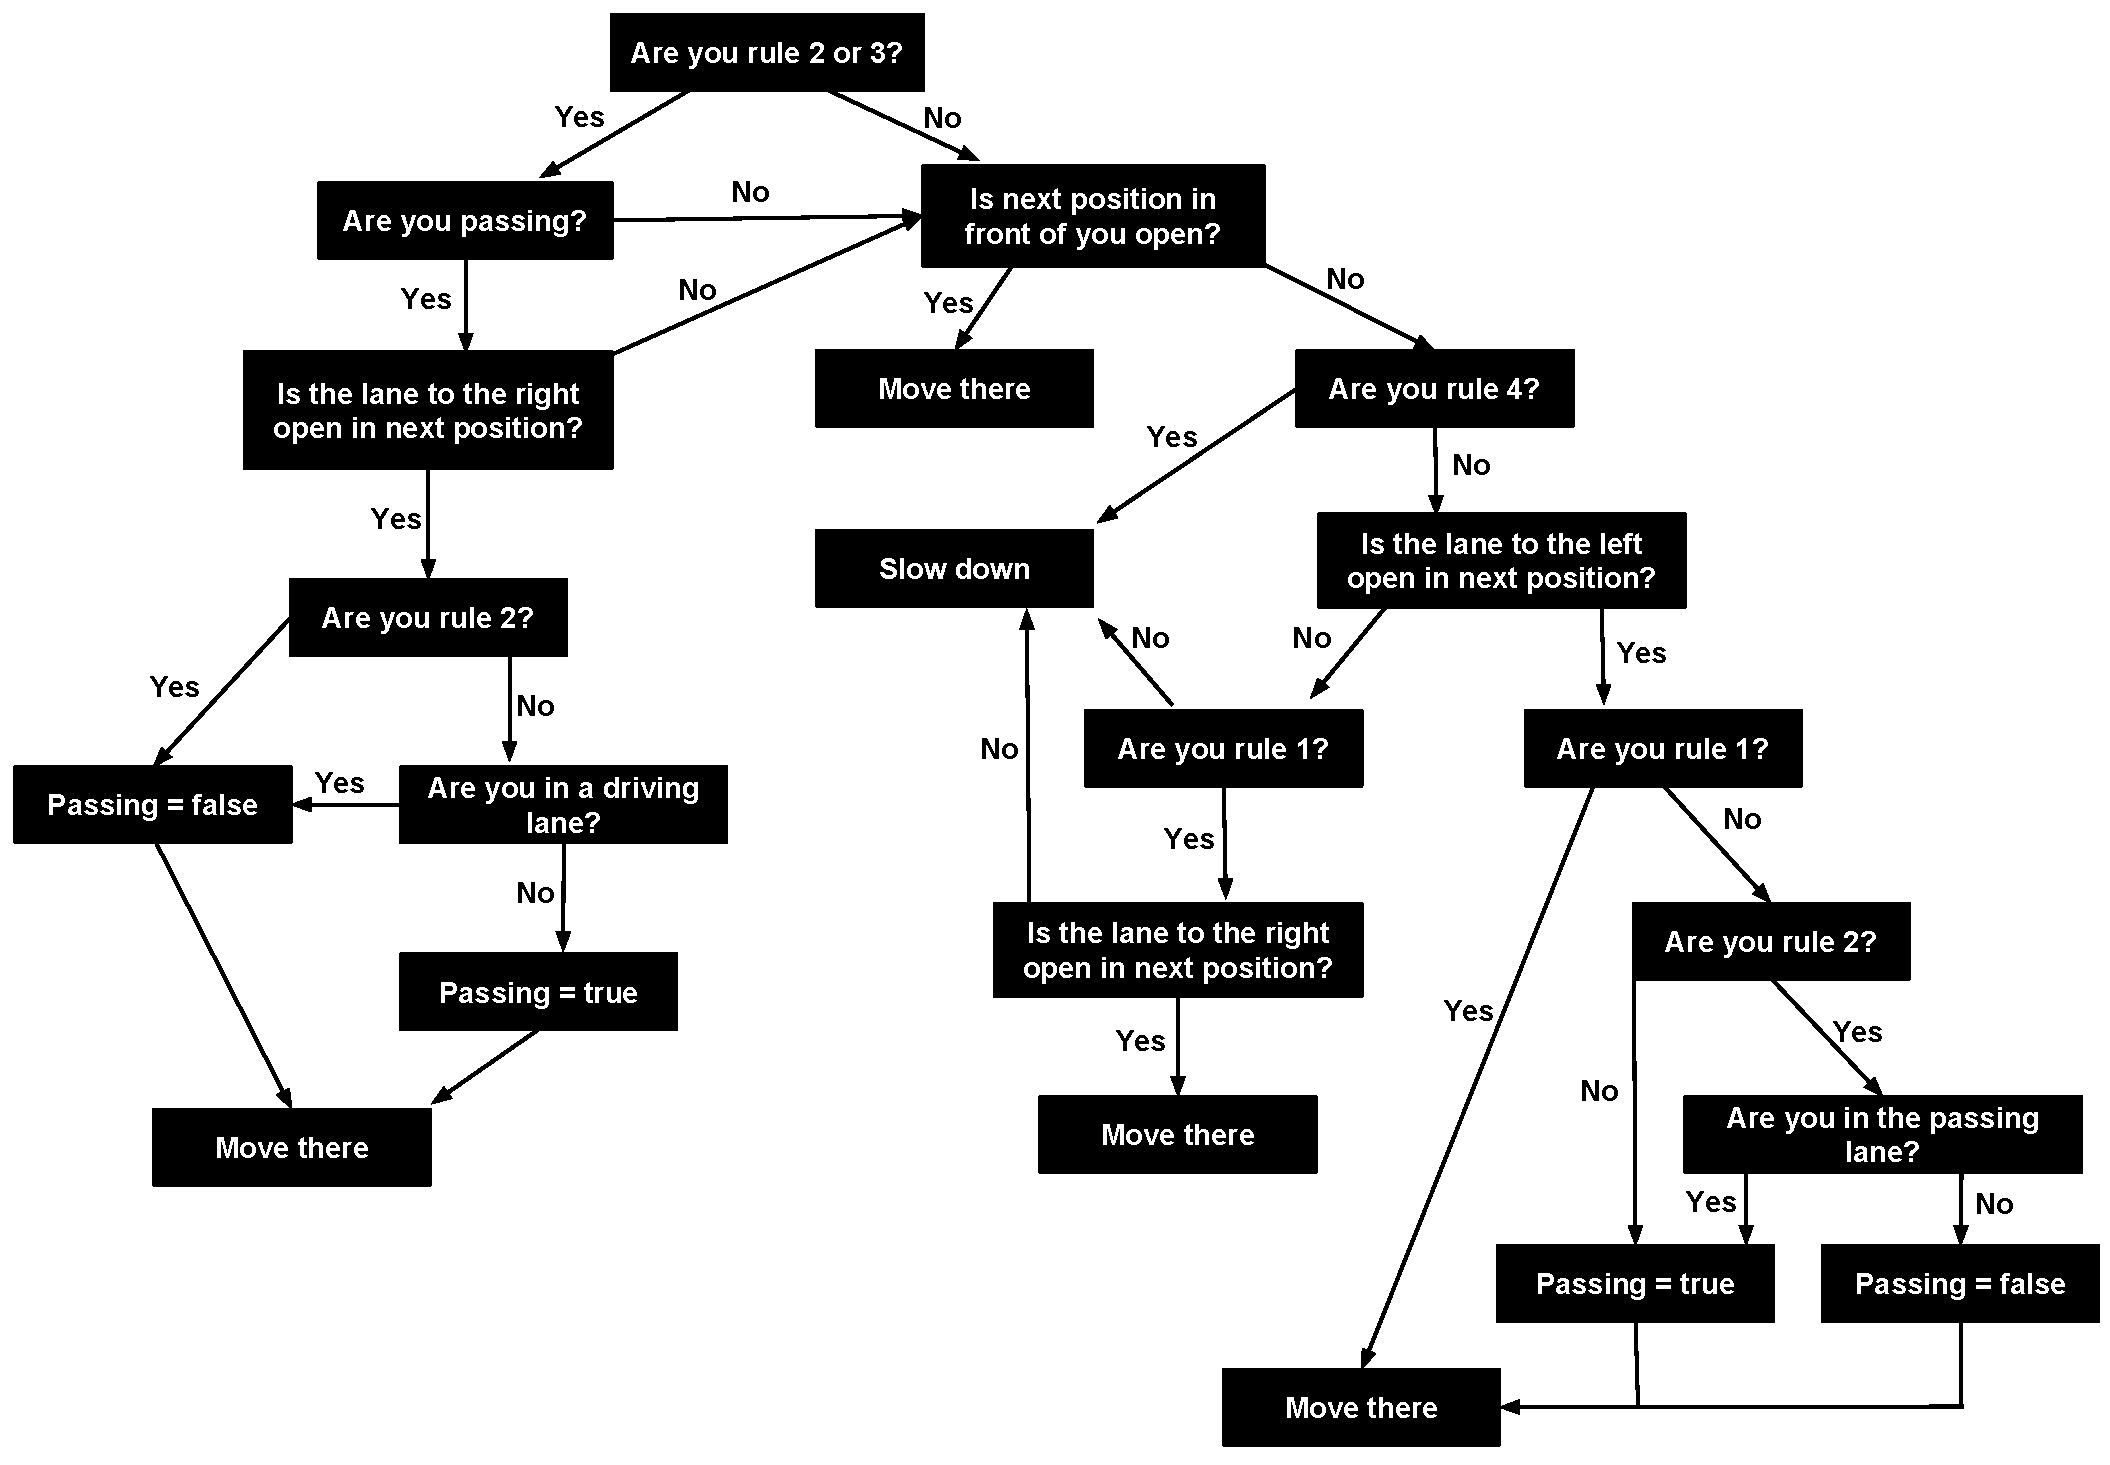
\includegraphics[scale=0.36]{MCM-LogicalFlowChart.pdf}
	\caption{The Logic Flow Chart of the programming sequence.}
	\renewcommand{\figurename}{}
\label{MCM-LogicalFlowChart}
	\end{center}	
	\end{figure}
	
	
	
	
	
	
\begin{figure}[h]
\begin{center}
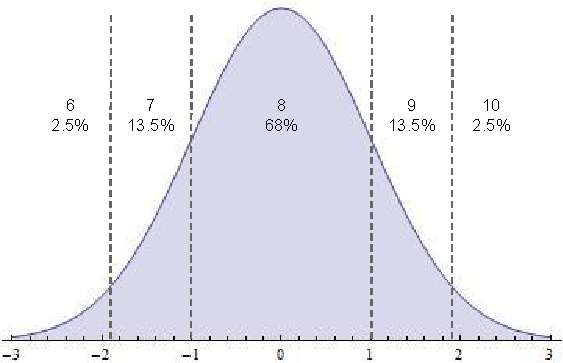
\includegraphics[scale=0.65]{MCM-speedsnormaldist}
\caption{Normal distribution graph of initial speed.}
\renewcommand{\figurename}{}
\label{MCMNormDist}
\end{center}
\end{figure}
		
\begin{figure}[h]
\begin{center}
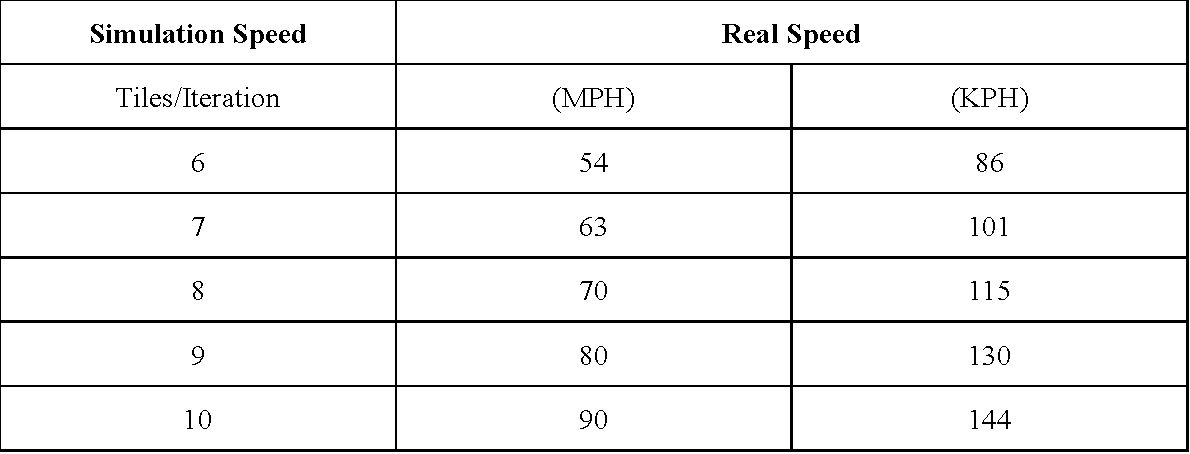
\includegraphics[scale=0.5]{MCM-SimulationSpeedTable.pdf}
\caption{Comparison scale of speed within model to the representation in real speeds.}
\renewcommand{\figurename}{Speed Scaling}

\end{center}
\end{figure}	
	
	
	
	
	
	
	
	
	
	


	
	
	
	\subsection{Probabilty Functions}
		\textit{Uniform distribution of position and lane}
			Our model utilized a standard random function inheritances in the OOPL(objected oriented programming language) we used to simulate our model. In initializing the lanes and slot for each individual car in the model, the program used a uniform distribution to place the cars along the freeway in discrete positions for every rule and simulation considered. The purpose of this was to consider what a hot air balloon would actually see on a freeway from a fixed position and height when observed randomly. The affects of this assumption are considered later in the statistical summary of the data of our model. 

		\textit{Normal distribution of speeds} 
			To incorporate a more realistic simulation of what we intended to model, we designed a normal distribution to describe the initialization of every car at the beginning of the simulation (See Figure ~\ref{MCMNormDist}.)

		\textit{Probability of a Crash}
			In our model we only had two dynamics to allow for crashes due to interactions, namely from slowing down and from changing lanes. We initially intended to account for severity and probability of a crash to determine how traffic may be affected for any given rule and initial conditions but found that identifying an accurate probability for a crash due to slowing down or changing lanes proved more time consuming than originally thought and rejected the idea of considering severity. We also found difficulty in accounting for crash back ups in the coding and simulation of our model and determined it detracted from the actual test of which rule was better for light and heavy traffic. Our model then considered probability of an accident as merely a rating by which to determine the better rule based on certain output statistics of our simulation, particularly number of lane changes, number of times a car slowed down, and number of times a car failed a lane change due to our logic structure, i.e. there was a car in its way when attempting to switch lanes(see logic structure). The formulation for the probability of  a crash had the following assumption and equations:
			
			\underline{\textit{Assumption}}
			\begin{itemize}
				\item The probability of slowing down and changing lanes are independent
				\item The probability of getting in an accident and changing lanes which we defined as a side-swipe accident was dependent
				\item The probability of getting in an accident and slowing down due to cars in front of you which we defined as a rear- end collision was dependent
			\end{itemize}
			\underline{\textit{Events}}
			\begin{itemize}
				\item A= The event there is an accident
				\item S = The event a car has slowed down
				\item L = The event a car has changed lanes
				\item D = The event the car has to make a decision in the logic tree, i.e. slow down or change lane
			\end{itemize}
			\underline{\textit{Equations}}
			\begin{itemize}
				\item $P(A \cap S) = P(S)P(A|S)$ by the multiplication rule and dependence.
				\item $P(A \cap L) = P(L)P(A|L)$ by the multiplication rule and dependence.
				\item $P(S \cap L) = \emptyset$
				\item $P(A \cap D) = P\big(A \cap (S \cup L)\big)= P(A \cap L) + P(A \cap S)$ by deMorgan's law.
				\item $P(S) = \frac{X_S}{X_D}$
				\item $P(L) = \frac{X_L}{X_D}$
				\item $P(A|L)= .02$  by statistical data from the \cite{GovStats}.
				\item $P(A|S)= .204$ is to be determined by statistical data from the \cite{GovStats}.
			\end{itemize}
		
\section{\bfseries{Simulation Program Results}}

	Here is a tabular representation of the program's computational outputs:

\begin{figure}[H]
	\begin{center}
	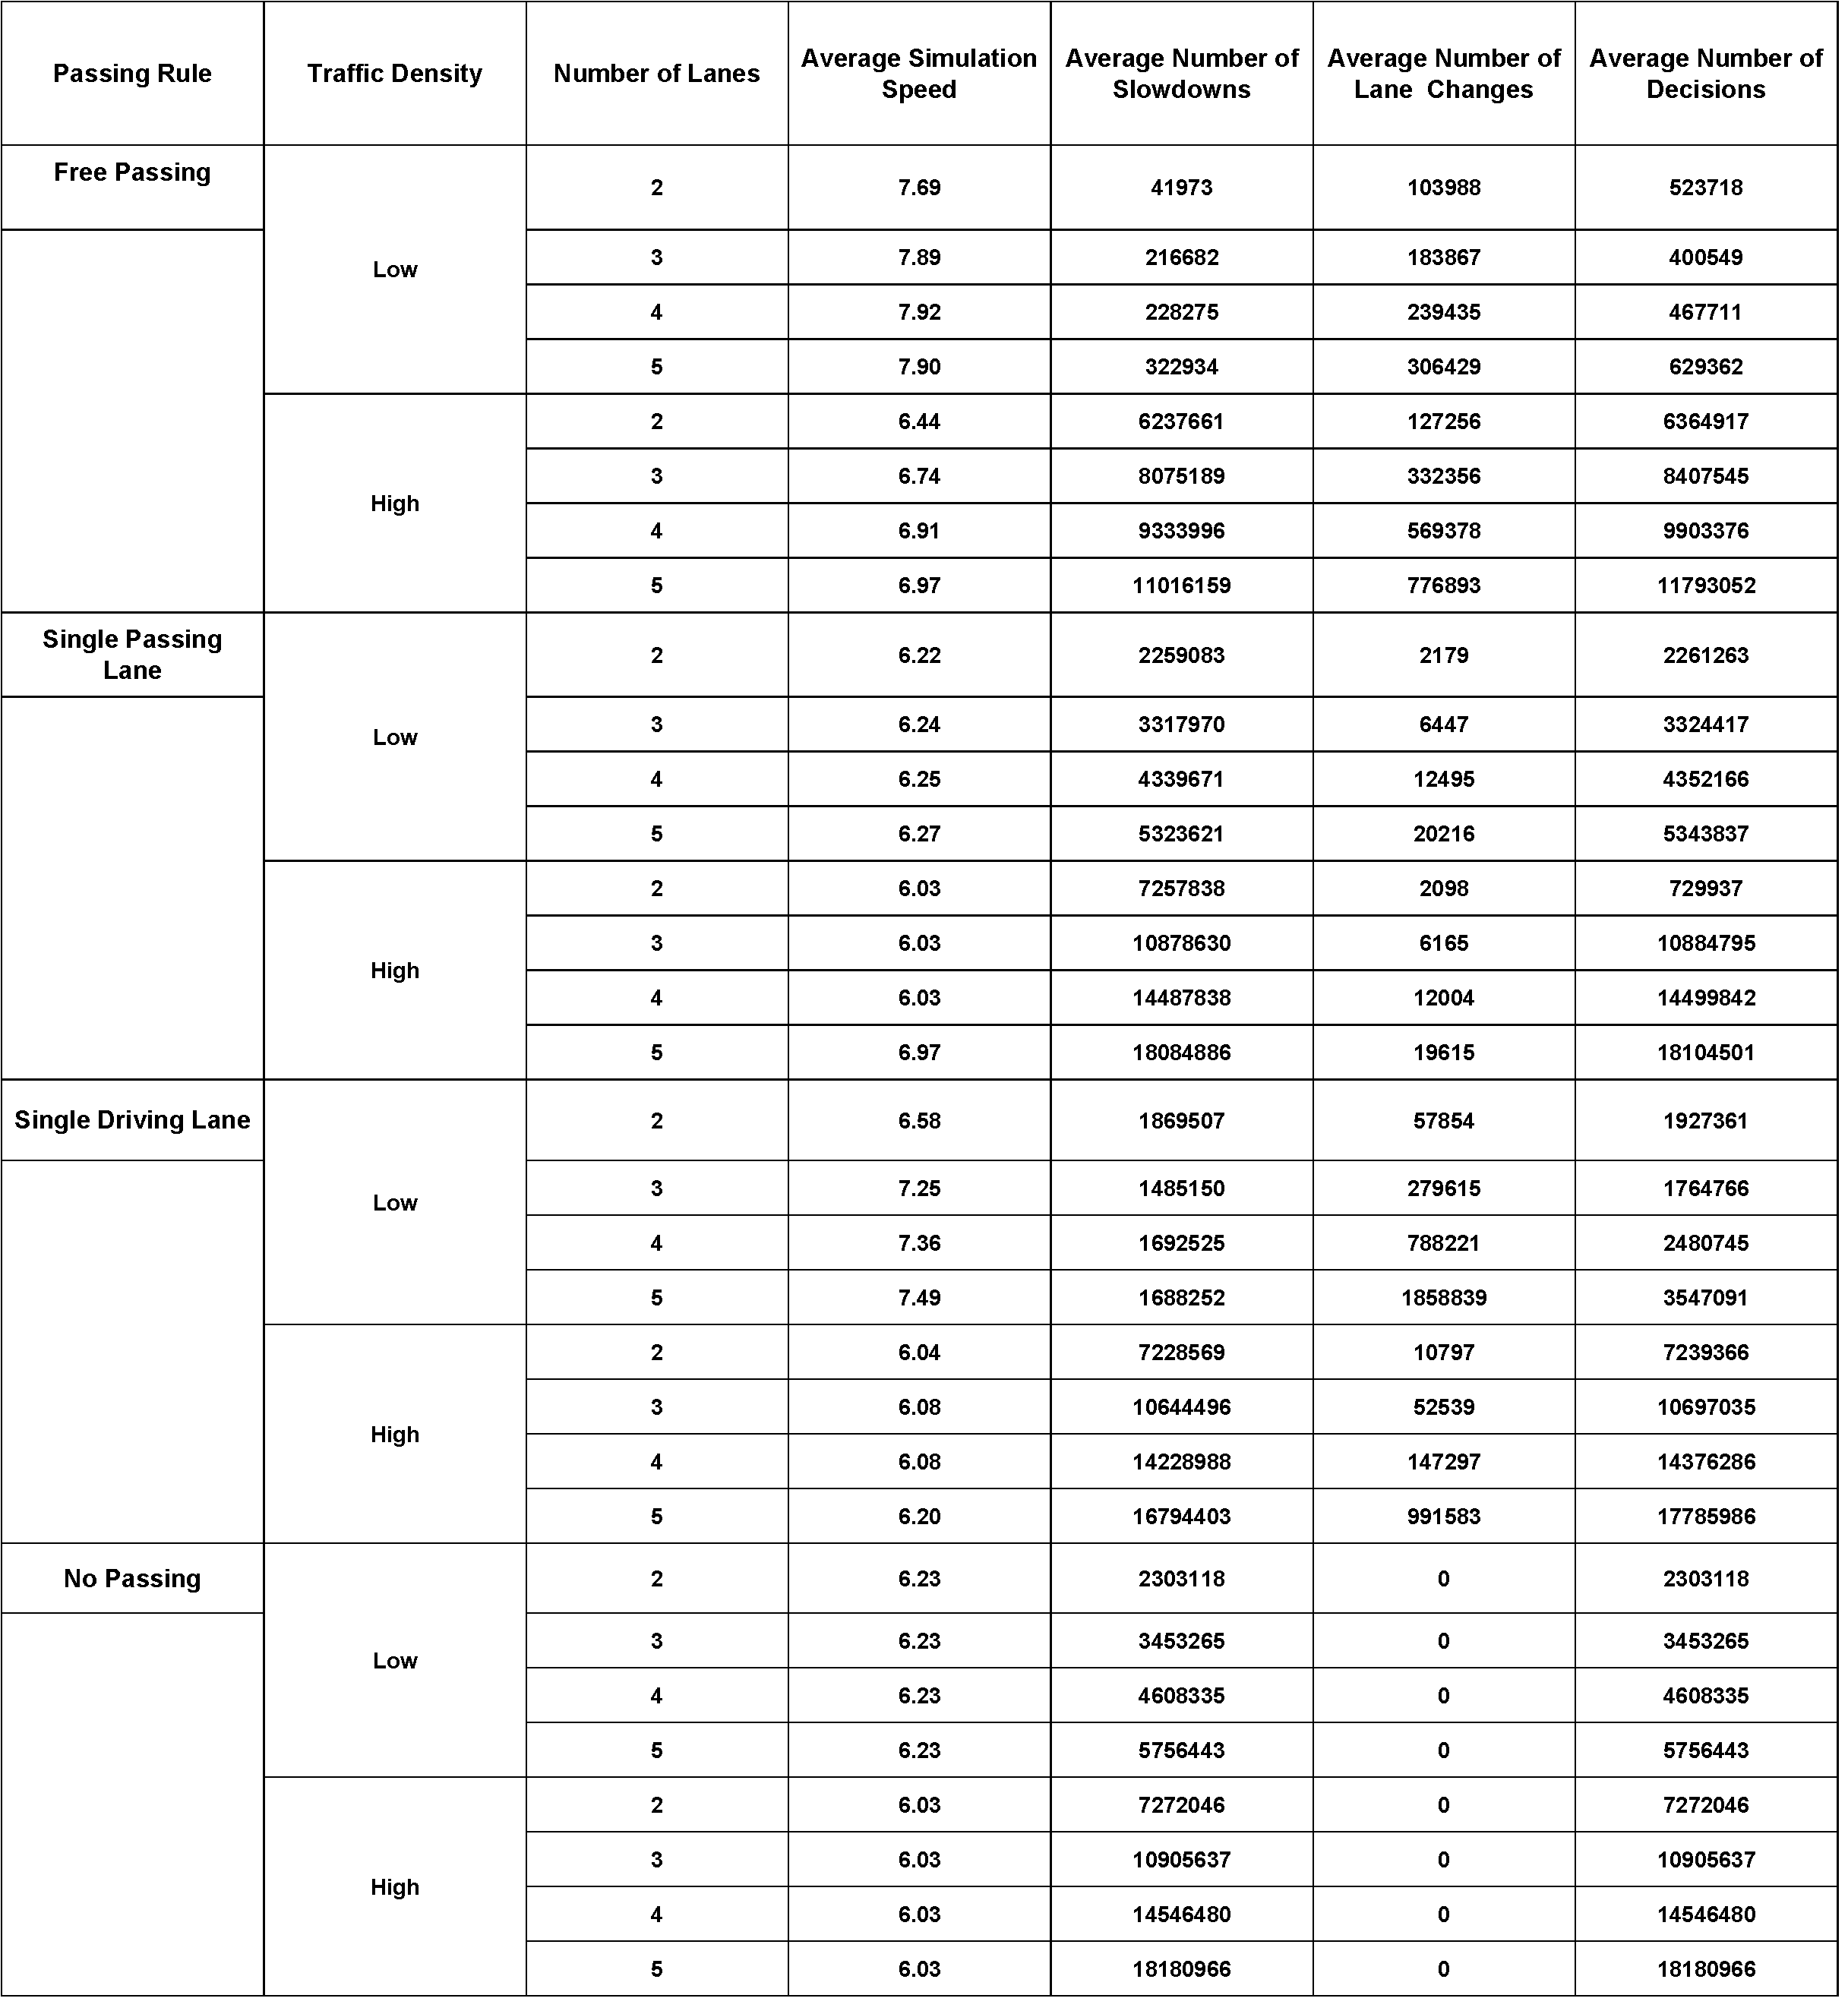
\includegraphics[scale=0.3]{MCMDataSummary}
	\caption{Program's computational outputs.}
	\renewcommand{\figurename}{}
	\end{center}
	\end{figure}

\section{\bfseries{Statistical Analysis}}
	In our analysis of the data, to determine which rule is best, we consider three factors,namely the average flow , the average number of accidents, and the average speed for a given simulation with initial conditions:
	\begin{itemize}
		\item Density of cars ( High or low)
		\item Number of lanes(2,3,4,5)
	\end{itemize}
	
	\subsection{Definitions}


	\begin{itemize}
		\item \textit{Population}: Every possibly value for the output parameters of our simulation.
		\item \textit{Parameter}: A characteristic of the distribution of our Population, such as its mean and variance.
		\item \textit{Sample Statistics}: Point estimates of the parameters of a given Simulation.
		\item \textit{Sample}: One complete run of all iterations for a set of initial conditions for a simulation.
		\item \textit{Control variables}: Parameters that stayed fixed for each road of the simulations, namely density and road length.
		\item \textit{Independent Variables}: The initial conditions used for each rode in a simulation.
		\item \textit{Dependent variables}:  Output sample statistics of the model.
		\item\textit{ Sample size}: Number of simulations ran for a specific set of initial conditions.
		\item \textit{Significance level}: The probability of rejecting a test hypothesis, $H_0$, incorrectly( i.e. Stating there is enough statistical evidence to support the alternative hypothesis,$H_a$, when in truth the the null or test hypothesis was correct). 
	
	\end{itemize}

	\subsection{Assumptions}
	\begin{itemize}
		\item Each simulation is independent of previous simulations.
		\item The best point estimates of mean traffic flow and mean speed of a simulation(Sample) is the sum of these quantities respectively, for each iteration over the number of iterations in a simulation.
		\item The optimal rule to implement in traffic based on our model is determined by the highest average traffic flow, highest average speed, and lowest average accident rate of the samples.
		\item Control variables will not affect determination of best rule
		\item A sample size of 30 will be enough to statistically consider our data in terms of a z-statistic for hypothesis testing
		\item A $95\%$ confidence level will be significant enough to cover the true population parameter of interest.
	\end{itemize}
	
	
	\textit{Justifications}
	
		We can assume each simulation is independent because the initial conditions have a random probability distribution associated with their discrete values and every simulation has no prior knowledge of previous simulations
	
		A Sample mean is the best unbiased estimate of the true value of a given population mean.

		Standard metrics of determining the implementation of particular highway policies are given be these sample statistics \cite{elvik2009handbook}.

		Many research papers use the simplifying assumption of conservation of cars, in order to find tractability in the model. Since this means that overall traffic density remains constant, we justify our assumption by considering the viewing space our model takes from a fixed position and fixed height over a highway during mid-day steady stream traffic \cite{seiboldconstructing}.
		By the central limit theorem, since we have the sample mean and variance and $n \geq 30$, we know we can approximate $W$ by $W=\frac{\bar x - \mu}{\sqrt{\frac{s^2}{n}}} \sim N(0,1)$.
		
		For reasonably centralized data $95\% $ significance is a strong test to use. The data being simulated by our model is only allowed to vary by some random independent variables and so the sample statistics are likely to show strong centralization. 
	
\newpage	
		
	\subsection{Z-Statistic Hypothesis Test Analysis}
	From our results we noticed that for nearly all road types the rule with the highest average of traffic flow, average simulation speed, and lowest safety rating was the free passing rule, while many of the other rules showed insignificant difference in simulation summary figures. However, one rule did standout from our results as a potential candidate to make a comparison with, the single driving lane.We tested the hypothesis that the free passing was indeed the best rule to implement based on our results. The single driving lane rule performed quite average in the low number of lanes simulations, but as lanes increased this rule seemed to demonstrate improvement in all three categories in consideration. Thus, we only performed hypothesis testing on these two rules. Our sample size was n = 30, which represented number of simulations whose summary data we averaged over all the samples. When testings the difference of two sample means, as long as the criterion that $n \geq 30$ is met, we can  reasonably approximate the sampling distribution as a Normal model which mean 0 and standard deviation 1. Hence, for the sample statistics $\bar q$ and $\bar v$ we can prove whether free passing is truly the best rule for all cases. For reference, the one-tailed hypothesis test and test statistic we used was the difference of means z- statistic with large sample size($n\geq30$) \cite{FundTrafficEng}: 	
	\begin{align*}
		H_o : &\mu_1 - \mu_2 \leq 0\\
		H_a : &\mu_1 - \mu_2 >0\\
		z_0 = &\frac{(\bar x_1 - \bar x_2) - (\mu_1 - \mu_2)}{\sqrt{\frac{1}{n}(s_1^2 + s_2^2)}}
	\end{align*}
	
	The $95\%$ confidence level determines the rejection region we will use, in particular we will reject the null hypothesis for test values of z which are greater than 1.645, formally:
	\begin{align*}
		R.R. = \{ z | z>1.645\}
	\end{align*}
\begin{figure}[H]
	\begin{center}
	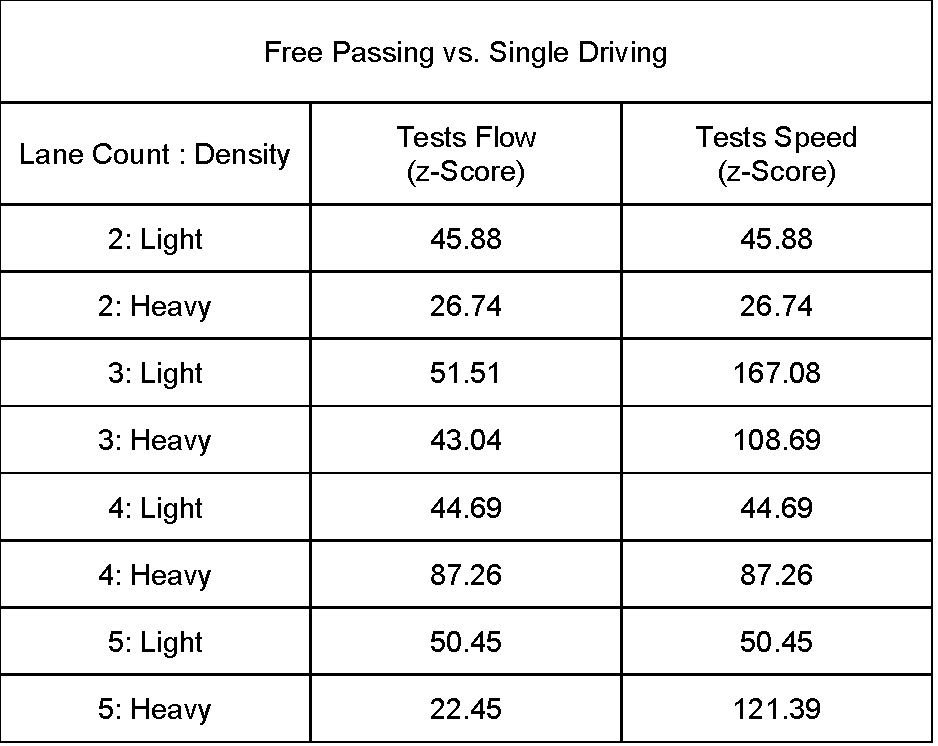
\includegraphics[scale=0.4]{MCMProbablityZ}
	\caption{One Tailed Difference of Means Z-Statistic Hypothesis Test}
	\renewcommand{\figurename}{}
	\end{center}
	\end{figure}
	
\newpage

	\subsection{Statistical Summary}A table of our sample statistics is provided below:
	
	\begin{figure}[H]
	\begin{center}
	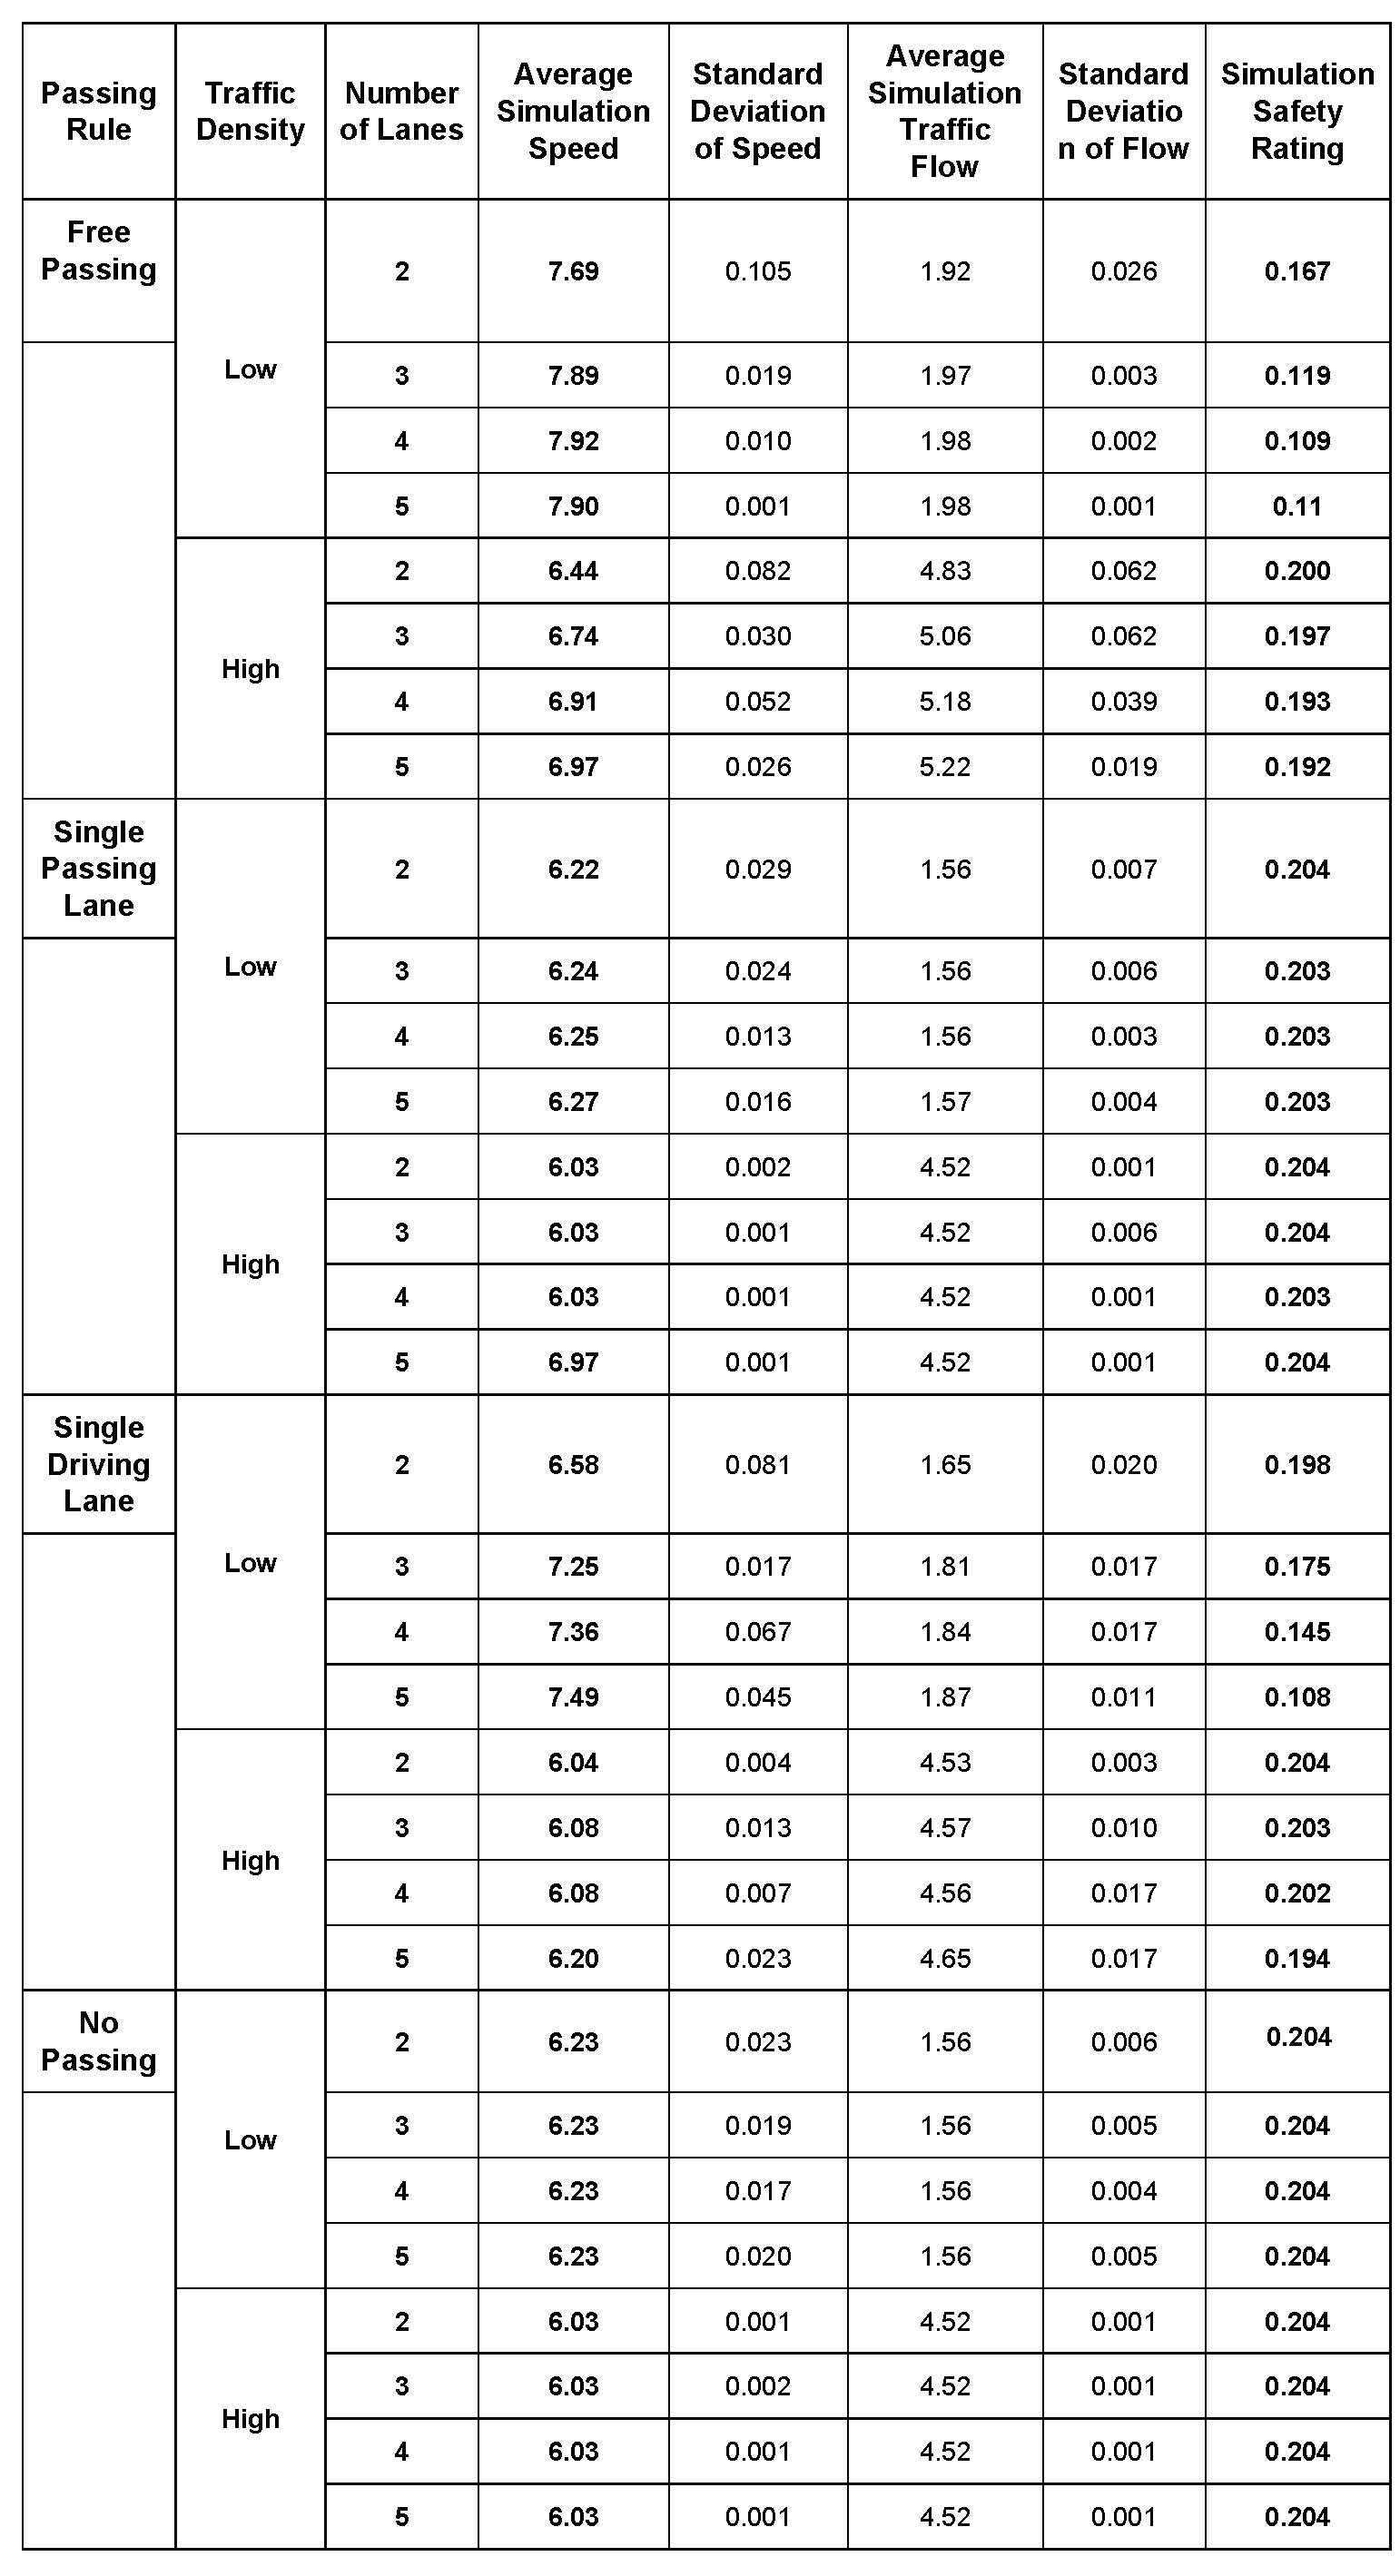
\includegraphics[scale=0.25]{MCMStatisticalAnalysisOfTrafficFlow}
	\caption{Calculated Statistical Data}
	\renewcommand{\figurename}{}
	\end{center}
	\end{figure}
	

	From our analysis we determine in the simulations of lanes 1 through 4 with low density and 1 thorough 5 with high density, the sample statistics for the free passing rule was significantly better then the rest. In fact, performing a p-value test on just one case, that is, measuring the probability of finding a more extreme value than z, we find 
	\[
		P( z > z_0) = 6.83 \e{-460}.
	\]
	This is a clear indication there is a flaw in our model because values this extreme are not only incredibly unlikely but too significant to consider as credible evidence. We believe the error could be contained in how the statistics are drawn from each simulation or how the program steps through its logic decision loop.  Because of this we determine our hypothesis testing of the sample means $\bar q$ and $\bar v$ are inconclusive. This may be due to a variety of influential factors,but we believe there is a very strong likelihood that these results stem from the minuscule standard deviations of the sample statistics. However, these were not the only characteristics in determining an optimal rule, we are still left with the simulation safety rating of each rule. From our statistical analysis summary above we see that free passing still was the dominant rule in terms of most safe, i.e. smallest safety rating, nevertheless the single driving still persists and proves to be the safest rule when the simulation has 5 lanes and low density.  

	\subsection{Statistical Analysis Difficulties}
	The data formatting was the most difficult part in the statistical analysis. At first we attempted to analyze the data on a iterations basis for each simulation by summing over the average iteration speed and dividing by 500, the total number of iterations. However in the XML(Extensible Markup Language) format that we used for persisting data, calculating the average of these iteration velocities for every simulation proved to be too difficult and time consuming in excel without using some type of XML to excel macro, which we were unskilled in. We did however achieve to find the sample statistics of average safety factor, average simulation velocity, and average traffic flow for a single road type, the 2 lane low density initial conditions. To overcome this unforeseen difficulty, we went back to the model in our object-oriented programming language and performed the simulation summaries which calculated the sample statistics for each simulation at that data type level rather than the iteration level, which minimized the time to determine the averages over all our samples that was used for our statistical analysis.


\section{\bfseries{Strengths and Weaknesses}}
	\subsection{Strengths}
		Our model took a unique approach to a problem which few other researches have truly considered. The modeling of a particle model for dynamics of a macro system is extremely elusive in finding tractable assumptions to make realistic solutions. The strengths of our model is that we attempted to put each of its elements into practical and concrete situations that explains its place in real life and  provide a frame work to build other concept on top of. The amount of contactable data about the model from the simulation can provide insights into a multitude of other questions which we have full intent to investigating. Another strength in the assumptions we made is that a simple switch of orientation would provide exactly the same outcome so further simulation is not needed, our logic based decision tree is non-oriented and so allows for direction to be changed regardless of rules implemented.
	\subsection{Weaknesses}
		A major set back of our model was its inability to accurately and definitively provide conclusive proof that a particular rule was better than all others within reason. This drawback did not prevent our ability to draw other conclusions from the model and indeed we now know what types of considerations must be taken, namely direct observation of parameters should always be preferred over averages of summary information. Furthermore, our limited time prevented us from implementing a mixed rule model which ideally would represent freedom of judge for a given simulation and parameters. Information about how such a system would behave can still be drawn from behavior of our current system, however our model's strict adherence to a specific rule seems more representative of an intelligently controlled traffic system. 
\section{\bfseries{Conclusion}}
	In conclusion, we believe our simulation was successful in modeling traffic dynamics in order to answer the question of how the stay-right-rule except to pass in light and heavy traffic. Many of the assumptions made were independently verified by external sources and proved to show effective dynamics in varying conditions. We found that there was limited trade off between traffic flow and safety and in fact, it was often the systems with the best traffic flow were the safest as well. We infer this is because freeways which are more congested, i.e slower traffic flow, have a higher probability of an interaction which results in an accident irrelevant of traffic density. Hence based on our model, we conclude that traffic flow and the probability of getting in an accident are inversely proportional to the extent that the average speed of the system does not approach grid lock. Furthermore, we found that number of traffic lanes plays a unique role in the dynamics of the rule and whether it works in various traffic densities. In particular, the stay-right-rule which we defined as the single driving lane rule became more effective in terms of average speed, average flow rate, and safety factor. We deduce this is due to the mechanics of the logic system it follows in which, the rule prefers open spaces in order to best cascade around cars and then collapse back to a single lane. We further predict that as we watch this segment of cars go indefinitely, due to the looping from the conservation of cars assumption we believe formation of packs should begin to emerge and will eventually reach complete segregation by the time our iterations of watching reaches infinity. Our final words are that traffic dynamics are challenging and intriguing. We have learned that often in modeling a situation, it is helpful to make assumptions of systems that are already known and simplify their models in order to match the problem you wish to consider, however other times it is best to originate a completely new idea and test its outcomes against known models that exists. 
	

	
	


\section{\bfseries{Future Work}}
	With the development of our program there are opportunities to adjust the starting conditions and individual vehicle interactions.  Therefore the programs parameters can be changed in order to make the model more practical to the real world or to test different traffic flow questions.  With this ability in our model some variations should be tested but could not be completed within the time frame.  
	\subsection{Car Individualized Rules}
	In our model we defined road rules where everyone on a highway followed the same set of passing rules.  This was a simplification assumptions in order to increase both programming and analysis time.  The problem here is that slow cars have the ability to start in the fast lanes and can get stuck there for a prolonged time.  Situations as slow cars in fast lanes does happen in real situations but not in the large scale that our model allows it. 
	The big variation that would be further followed would be to assign individual vehicles a passing rule instead of everyone on the same highway a passing rule.  This highly increases the realism of our model since every driver has their own average speed they tend to travel.  Furthermore, this implication would help diminish the intelligent design factor that has overrun our program.  In our current model everyone follows the rule no matter the interaction.  This insistence to follow the passing rule would be still upheld in the individualized car passing rules but by varying what type of rules are seen on a highway we can model a more realistic road.  
	
	\subsection{Psychology Driver Variation}
	One model found attempted to test individual driver psychology of driving.  This acts as a subdivision of the varying speed adjustment.  Driver's may be influenced by perceived safety, age, likelihood to be distracted, emotional distress, etc.  Furthermore in this psychology of individual drivers there is the consideration that drivers can only perceive in a limited viewing frame and thus only varying their speed by the vehicles around them ~\cite{burghout2005}.  These are attributes that cannot easily be incremented into our program but would be interesting to pursue if with a small set of simple assumptions our program could begin to describe some of these variations.     


\newpage
\section{\bfseries{References}}
\bibliography{References}











\end{document}
